% TEX root =  lfgw-beamer.tex
% !TEX root =  lfgw-article.tex
% !TEX encoding = UTF-8 Unicode
% !TEX TS-program = pdflatex

%
% Schriften
%
\usepackage[TS1,T1]{fontenc}
%\usepackage{charter}	\renewcommand{\sfdefault}{bch} % not in small
%\usepackage{utopia}	\renewcommand{\sfdefault}{put} % not in small
%\usepackage{lmodern}
%\usepackage{dejavu}
\usepackage{libertine}
%\usepackage{PTSans}

%\usepackage{eurosym}
%\usepackage{ccicons}

% Literaturverzeichnis mit Biblatex
%
%\usepackage[style=alphabetic,hyperref,backend=biber]{biblatex}
%\usepackage[style=numeric-comp,hyperref,backend=biber]{biblatex}
%\bibliography{HS} % Literaturdatenbank (ohne biblatex am Ende)
%
%\usepackage{csquotes}	% Wird für biblatex benötigt. % not in small

\title{Präsentationen mit Beamer}
%\subtitle {Untertitel} % (optional)
\author{Axel Kielhorn}

\begin{document}

%\mode<presentation>{
%%\setbeamertemplate{background}{\includegraphics[width=\paperwidth]{HD_back}}
%\usebackgroundtemplate{\includegraphics[width=\paperwidth]{HD_back}}
%}
\begin{frame}<beamer>[plain,b,label=mitmachen] % b = bottom

\huge\bfseries\color{structure!20} %Text auf Titelseite

Eine Musterpräsentation

\vspace*{7.1cm}

\end{frame}

\mode<presentation>{
%\setbeamertemplate{background}[default]
\usebackgroundtemplate{}
}

%%% Ende ignorieren

\begin{frame}<beamer>[<*>][label=titel]{}
  \titlepage
\end{frame}

\maketitle

\begin{frame}[label=vorspiel]{Vorspiel}
  \begin{itemize}[<*>]
    \item Zwei Steuerdateien für 
      \begin{itemize}
        \item Präsentation und
        \item Handout.
      \end{itemize}     
    \item Eine Inhaltsdatei enthält Folien (Frames) und zusätzliche Kommentare.
  \end{itemize}
\end{frame}

\section{Templatesuche}
\subsection{Vorlage}
\begin{frame}[label=theme]{Themes}
   \begin{itemize}[<*>]
  \item
    Einfaches Themes
  \item
    Themes mit Section und Subsection
  \item
    Einfaches Themes mit Navigationszeile
  \item
    Themes mit Navigationsrahmen
  \item
    Themes mit Inhaltsverzeichnis
  \end{itemize}
\end{frame}

Für einige Universitäten und Firmen gibt es bereits fertige Templates.
Es lohnt sich im Internet danach zu suchen. (Oder in der TeXLive-Installation.)

\subsection{Farbe}
\begin{frame}[label=farbe]{Farbwahl}
%  \setbeamersize{description width of ={{Pointless Albatross}}}
   \begin{description}[<*>]
  \item[Spruce]
    Dezent
%  \item[Pointless Albatross]
  \item[Albatross]
    Aufdringlich
  \item[Beetle]
    Seriös
  \item[Crane]
    Freundlich
  \item[Dove]
    Sehr zurückhaltend
  \end{description}
\end{frame}

Hell oder Dunkel ist nicht nur Geschmackssache.
Da Präsentationen selten unter optimalen Bedingungen gehalten werden, 
kann es sinnvoll sein, eine helle und eine dunkle Präsentation vorzubereiten.
So kann man bei schlechten Lichtverhältnissen schnell auf eine Alternative wechseln.

\subsection{Schriften}
\begin{frame}[label=schrift]{Schriftwahl}
   \begin{itemize}[<*>]
  \item
    Größe: 8 pt bis 17 pt
  \item
    Mit Serifen: Charter, Utopia,  \dots
  \item
    Serifenlos: Latin Modern, DejaVu, PTSans, \dots
  \end{itemize}
\end{frame}

\section{Inhalt}
\subsection{Rahmen}
\begin{frame}[label=rahmen1,fragile]{Rahmen}
  \begin{verbatim}
    \begin{frame}{Rahmen}
     Inhalt
    \end{frame}
    
    \frame{
          \frametitle{Rahmen}
          Inhalt
          }
  \end{verbatim}
\end{frame}

\begin{frame}[label=rahmen2,fragile]{Rahmen mit Overlayspezifikation}
  \begin{verbatim}
    \begin{frame}<beamer>{Inhalt}
    % Nur im Beamer-Mode anzeigen 
       \tabelofcontents[pausesections]
    \end{frame}
  \end{verbatim}
\end{frame}

\begin{frame}<beamer>[label=inhalt]{Inhalt}
    % Nur im Beamer-Mode anzeigen 
    \tableofcontents[pausesections]
    %\tableofcontents[currentsection] % nur aktuelle Section
\end{frame}

\subsection{Inkrementell}

Natürlich nur in der Präsentation, im Artikel erschein alles auf einmal.
Vorsicht wenn Texte in der Präsentation ersetzt werden.

\begin{frame}[label=inkrementell1]{Inkrementell}
  \begin{itemize}[<+->]
    \item Erstens
    \item Zweitens
    \item Drittens
    \only<article>{Nur im Handout}
  \end{itemize}
\end{frame}

\begin{frame}[label=inkrementell2]{Inkrementell manuell}
  \begin{itemize}
    \item <1->Erstens
    \item <2->Zweitens
    \item <3->Drittens
    \item <3->"`Drittens"' in einer postsekundaren Gesellschaft
  \end{itemize}
\end{frame}

\begin{frame}[label=inkrementell3]{Inkrementell alternativ}
  \begin{itemize}[<+->]
    \item Erstens
    \item Zweitens
    \item Drittens
    \item <.->"`Drittens"' in einer postsekundaren Gesellschaft
  \end{itemize}
\end{frame}

\begin{frame}[label=inkrementell4]{Inkrementell}
    \begin{block}{Erstens}
    Nicht vergessen!
    \end{block}
    \begin{alertblock}{Zweitens}
    Unbedingt dran denken!
    \end{alertblock}
    \begin{exampleblock}{Drittens}
    Sehr wichtig!
    \end{exampleblock}
\end{frame}

\begin{frame}[label=inkrementell5]{Inkrementell horizontal}
  \begin{tabular}{llrrr}
    Kernal 	& Wert 		& Wert 2 	& \uncover<2>{Wert 2} \\
    		&		&		& \uncover<2>{optimiert}\\
    2.7		& $0.85$ 	& 39\% 		& \uncover<2>{ 35\%}\\
    2.7		& $0.95$ 	& \alert<2>{49\%} 		& \uncover<2>{\alert<2>{ 44\%}}\\
    2.7		& $0.98$	& 55\% 		& \uncover<2>{ 51\%}
  \end{tabular}
  
  %\hyperlink<3>{Bilder}{\beamergotobutton{Zu Bilder springen}}
  %\hyperlink<3>{Bilder}{\beamerskipbutton{Zu Bilder springen}}
\end{frame}

\begin{frame}[label=inkrementell6]{Mehrspaltig}%<beamer>
\begin{columns}[t]
\begin{column}<1->{0.5\textwidth}
Es ist so eng hier. Muss man das denn unbedingt zweispaltig setzen?
\end{column}%
\begin{column}<2->{0.5\textwidth}
Ich will raus!
\end{column}
\end{columns}
\end{frame}

\subsection{Übergänge}
\begin{frame}[label=trans]{Seitenwechsel}
\setbeamersize{description width of ={{transblindshorizontal}}}
  \transblindsvertical
  Beamer unterstützt animierte Seitenwechsel, jedoch nur
  bei Verwendung von Acrobat Reader im Vollbildmodus.
  \begin{description}
    \item[transdissolve] Eine Seite löst sich in Punkten auf und eine neue entsteht
    \item[transblindshorizontal] oder vertical
    \item[transboxin] oder boxout
    \item[transwipe] I am the Wiper
  \end{description}
\end{frame}

\subsection{Bilder}
\begin{frame}<beamer>[label=bilder1]{Bilder}
   \hypertarget{Bilder}{}
   \includegraphics[keepaspectratio=true,width=1\textwidth]{Facebookspiel.png}
\end{frame}

% Nicht bei Seitenleiste
%
\begin{frame}[plain,label=bilder2]
  \begin{centering}%
    \pgfimage<beamer>[width=1\paperwidth]{Facebookspiel.png}%
    \pgfimage<article>[width=1\textwidth]{Facebookspiel.png}%
    \par%
  \end{centering}%
\end{frame}

% Passt immer (2 TeX Läufe) nicht für article
%
\begin{frame}<beamer>[plain,label=bilder3]
   \begin{tikzpicture}[remember picture,overlay]
      \node[at=(current page.center)] {\pgfimage[width=1\paperwidth]
      {Facebookspiel.png}};
   \end{tikzpicture}
\end{frame}

\mode<presentation>{
  \setbeamercovered{invisible}
}

\begin{frame}[fragile,label=tikz]{Tikz}
   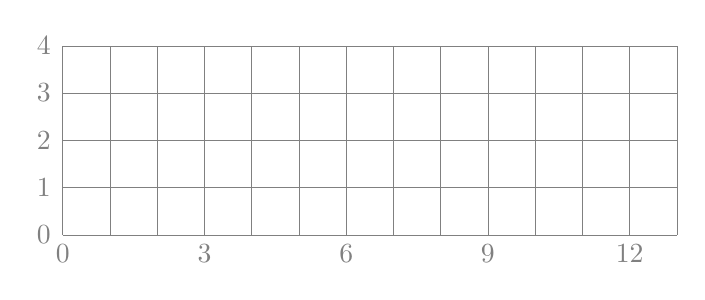
\begin{tikzpicture}[scale=0.6]
   \draw[help lines] (0,0) grid (13,4);
   \draw[gray] (-0.4,0) node {0} (-0.4,1) node {1} 
               (-0.4,2) node {2} (-0.4,3) node {3} (-0.4,4) node {4};
   \draw[gray] (0,-.4)  node {0} (3,-.4)  node {3} 
               (6,-.4)  node {6} (9,-.4)  node {9} (12,-.4) node {12};
      \pgfplothandlerlineto 
      %\pgfplotxyfile{facebook.dat}
      \onslide<2>\pgfplotxyfile{facebook.dat}
      \pgfusepath{stroke}
   \end{tikzpicture}
\end{frame}

Wie funktioniert das Facebook Spiel?
Ein Rentner meldet sich bei Facebook an und findet dort drei seiner alten Freunde.
Nach 6 Monaten stirbt der erste.
Nach 9 Monaten stirbt der zweite und nach 13 Monaten der letzte.
Sieger!

%\nocite{*} % alle Angaben in bib Datei ausgeben
%\printbibliography

\end{document}

